%pre-processing
\subsection{KHT}
As claimed in Section 2, given a query q it is sufficient to only tackle the relevant objects in $RO_q$, due to other objects have no contribution to satisfy the users' needs. To alleviate the unnecessary computation and boost the search efficiency, in this section, we introduce the keyword hash table (KHT) index, which is organized as a hash table with \textbf{\textit{perfect hashing technique}}.
\begin{table}
\centering
\begin{tabular}{|l|l|l|c|c|}
\hline
Entry &Keywords & OList & FI & SI \\
%OID & Position_x & Position_y & Associated keywords \\
\hline \hline
$e_1$ &$mountain$ & $o_1,o_3,o_7,o_{10}$ & 5 & 0\\
\hline
$e_2$ &$forest$ & $o_3,o_9$ & 6 & 1 \\
\hline
$e_3$ &$landscape$ & $o_1,o_7$ & 6 & 2 \\
\hline
$e_4$ &$shore$ & $o_2,o_4,o_5$ & 6 & 1 \\
\hline
$e_5$ &$temple$ & $o_1,o_3,o_6$ & 1 & 0 \\
\hline
$e_6$ &$museum$ & $o_2,o_7$ & 2 & 0 \\
\hline
$e_7$ &$architecture$ & $o_5,o_6$ & 5 & 1 \\
\hline
$e_8$ &$drigtate$ & $o_5,o_{10}$ & 0 & 0 \\
\hline
$e_9$ &$glacier$ & $o_8,o_{10}$ & 4 & 0 \\
\hline
\end{tabular}
\caption{$KHT$ entries}\label{T4}
\end{table}

In a nutshell, the KHT consists of two major components:
\begin{itemize}
    \item Distinct keywords: A vocabulary of all the distinct keywords appearing in the object database.
    \item OID list: For each distinct keyword $\lambda$, there is a posting list which records the $RO_\lambda$.
\end{itemize}

Each entry of KHT of the form $(\lambda,\lambda.olist, FI, SI)$, where $\lambda$ represents a keyword and $\lambda.olist$ is the $RO_\lambda$. $FI$ and $SI$ correspond to the first and second index of $\lambda$ in KHT. Table \ref{T4} elaborates the KHT entries, and Fig. \ref{F1} shows the KHT structure of Table \ref{T1}.

\begin{figure}
\centering
\includegraphics[width=3.5in,height=1.5in]{KHT}
\caption{The KHT instance} \label{F1}
\end{figure}

To balance the search efficiency and storage space, we combine the two-level index technique and perfect hashing technique \cite{cormen2001introduction} in our work. We assign each entry an index $(Fi,Si)$, with which we can retrieve a KHT entry in nearly $\Theta(1)$.

\begin{figure}
\centering
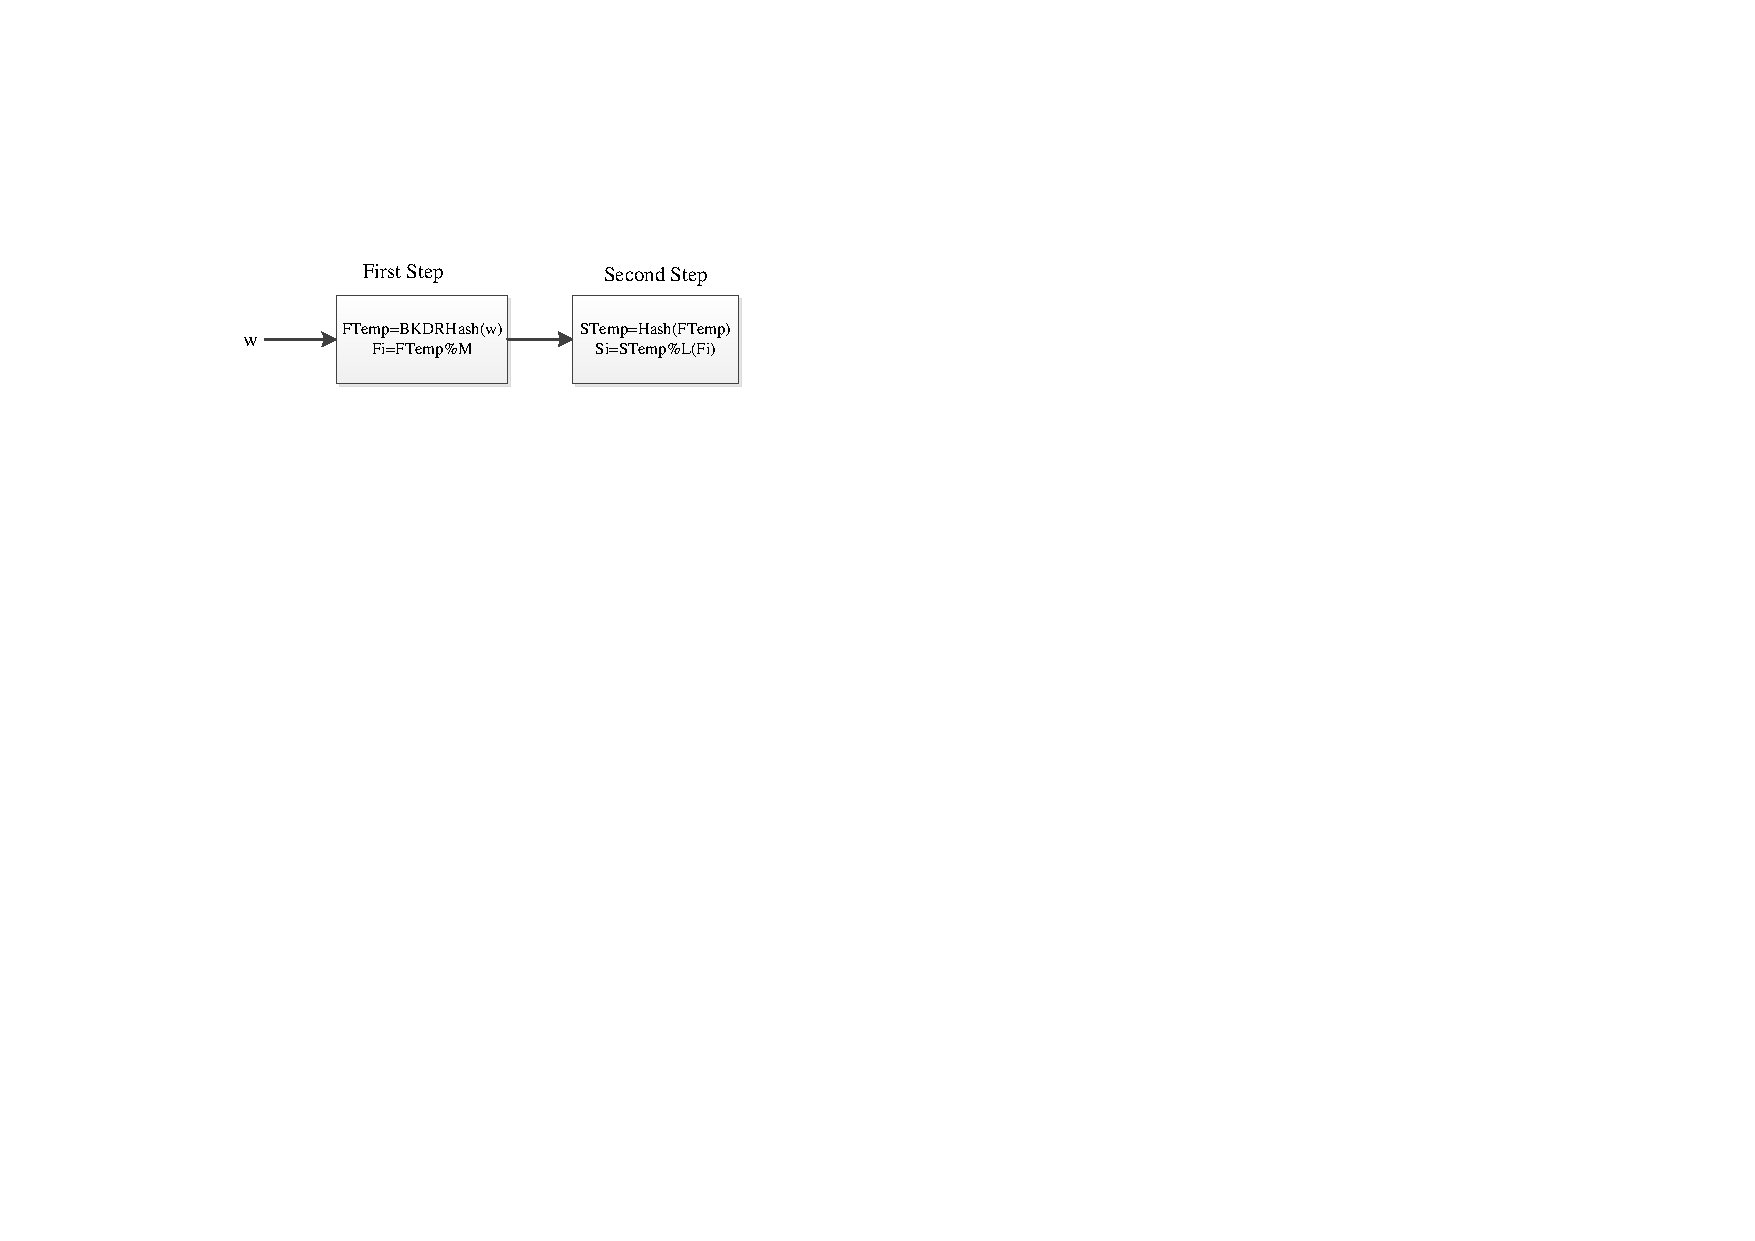
\includegraphics[width=3.5in,height=0.6in]{HASH}
\caption{The Hash Function} \label{F20}
\end{figure}

As illustrated in Fig. \ref{F20}, we determine the index of an entry in two steps. In the first step, we first map the keyword w of entry to the FTemp with the string hash function BKDRHash. It's worth to note that, although we apply BKDRHash as hash function, others string hash function can also be applied. And then, we obtain the $Fi$ by performing a modulus on FTemp with first-level index length M. In the second step, we hash the FTemp with an integer hash function and then perform a modulus on STemp with second-level index length of $Fi$ to get $Si$. After these two steps, each KHT entry has an index $(Fi,Si)$. Note that, a delicate situation arises when two or more entries share the same index $(Fi,Si)$ whose probability less than 0.5, which is demonstrated in \cite{cormen2001introduction}. In this case, \textbf{\textit{``linear probing''}} technique is utilized to tackle this problem. From Table \ref{T4} we know that there is a conflict situation between ``forest'' and ``shore''. As illustrated in Fig. \ref{F1}, when we try to insert the entry $e_4$ into KHT, $e_2$ has already stayed in location $(6,1)$. Due to location $(6,2)$ is occupied as well, with ``linear probing'', $e_4$ is inserted into $(6,3)$ ultimately, just as the solid arrow shown.

With KHT, for a specific query q we can retrieve the $RO_q$ in nearly $\Theta(|q.\omega|)$, and prune the unnecessary visits hugely.

\subsection{The Exact Algorithm MergeList}
For many real application scenarios, the number of query keywords submitted by users is limited. Motivated by this observation, we devise an exact algorithm MergeList in this section.

The straightforward method for the exact algorithm is to enumerate all the subsets of $RO_q$ and return the subset, which covers the query keywords not less than a given threshold and with minimum cost, as our optimal solution. This yields an exponential time complexity in terms of the number of objects in $RO_q$.

To further prune the search space, we delve into several efficient pruning strategies below.

Firstly, we sort the objects of $RO_q$ in ascending order of the cost distance. And we record the current optimal solution and its cost with notations $COS$ and $minCost$. Instead of enumerating all the subsets of $RO_q$ randomly, we construct the candidate subsets whose cost less than minCost by adding object into existing candidate subsets progressively.

\begin{lem}
    Given a sorted $RO_q$ which in ascending order of the cost distance. If for each existing candidate set \textbf{ecs}, the cost sum of ecs and the current visitorial object \textbf{cvo} in $RO_q$ is not less than minCost, then COS is the optimal solution.
    \begin{pot}
        Since $RO_q$ is sorted in ascending order of the cost distance. We know that each object behind cvo in $RO_q$ has a higher cost than cvo. If the cost sum of any ecs and cvo is not less than minCost, we can conclude that any ecs can not be the optimal solution, so we can terminate our procedure immediately.
    \end{pot}
\end{lem} \label{L5}

Secondly, there is an \textbf{\textit{``Apriori property''}} in the data mining field. \textbf{\textit{``All nonempty subsets of a frequent itemset must also be frequent''}}. In the sequel, we present a similar pruning strategy.

\begin{lem}
    If the cost sum of an ecs and cvo larger than the minCost, we can prune the ecs safely and any superset of it needs not to be computed.
    \begin{pot}
        If the cost sum of an ecs and cvo larger than the minCost, we know that ecs cannot be the optimal solution and any superset of ecs neither can be the optimal solution as well, so we can prune them safely.
    \end{pot}
\end{lem} \label{L6}

Further, only if G is a feasible solution, we can filter out any superset G', since G is superior to G' anyway.

In a word, Lemma 3 allows us to terminate the procedure earlier and Lemma 4 provides significant pruning ability. We elaborate the MergeList in Algorithm \ref{A4}.

The MergeList algorithm can be summarized as following three steps.
\begin{itemize}
    \item Step 1 (Construct $RO_q$): In this step, we construct the $RO_q$ and sort it in ascending order of cost distance.
    \item Step 2 (Add o into $ecs$): For object o in $RO_q$, we verify for each ecs whether delete it from candidate sets $SS$ or combine it with o and put it into $SS$.
    \item Step 3 (Iterative step): Repeat Step 2, until the terminal condition in Lemma 3 is met.
\end{itemize}

%The MergeList algorithm
\IncMargin{1em}
\begin{algorithm}[!hb]
\caption{$MergeList$} \label{A4}   % 给算法一个标签,以便其它地方引用该算法
%\DontPrintSemicolon
\SetKwInOut{Input}{Input}\SetKwInOut{Output}{Output}
\Input {The $KHT$ and the query $q$.}
\Output{A group $G$ of objects as resulting solution.}
\BlankLine
\LinesNumbered
$COS \longleftarrow \emptyset$\;
$SS \longleftarrow \emptyset$\;
$minCost \longleftarrow$ INFINITE\_MAX\;
$RO_q \longleftarrow$ compute the relevant object set to query q with $KHT$\;
sort $RO_q$ in ascending order of weight distance cost\;
put empty set ${\O}$ into SS\;
\For{each object $o \in RO_q$} {
    \If{$wd(o,q)\geq minCost$} {
        break\;
    }
    \For{each $ecs \in SS$}{
        \If{the cost sum of $ecs$ and $o$ not less than $minCost$} {
            delete $ecs$ from $SS$\;
            continue\;
        }
        $tempSet \longleftarrow ecs\cup \{o\}$\;
        \eIf{$tempSet$ is a feasible solution} {
            $COS \longleftarrow tempSet$\;
            $minCost \longleftarrow$ the cost of $tempSet$\;
            delete $ecs$ from $SS$\;
        } {
            put $tempSet$ into SS\;
        }
    }
    \If{$SS == {\O}$} {
        break\;
    }
}
$G \longleftarrow COS$\;
return $G$ as the final solution\;
\end{algorithm}
\DecMargin{1em}

As discussed above, in MergeList algorithm, we construct the candidate set by adding the object into ecs progressively. We use $SS$ to store the ecs, and initiate $SS$ with the empty set (line 6). For each object o in $RO_q$, if the cost of o not less than minCost then we terminate our procedure (lines 8-9). Otherwise, for each ecs satisfies Lemma 4, we prune it directly (lines 11-13). If $tempSet$ is a feasible solution, we use it to update the $COS$ and $minCost$ (lines 15-18), otherwise we add it into $SS$.

%\begin{table}[h]
%\centering
%\begin{tabular}{|c|c|c|c|c|c|}
%\hline
% OID & $o_1$ & $o_2$ & $o_3$ & $o_4$ & $o_5$\\
%\hline
 %Cost Distance to q& 2 & 2.5 & 4 & 5 & 7 \\
%\hline
% CP &0.1, 0.0&0.1, 0.3&0.3, 0.1&0, 0.3&0.1, 0.3\\
%\hline
%\end{tabular}
%\caption{An example of MergeList} \label{T6}
%\end{table}
\begin{figure}[!ht] \centering
    \subfigure[] { \label{MergeList-Q}
    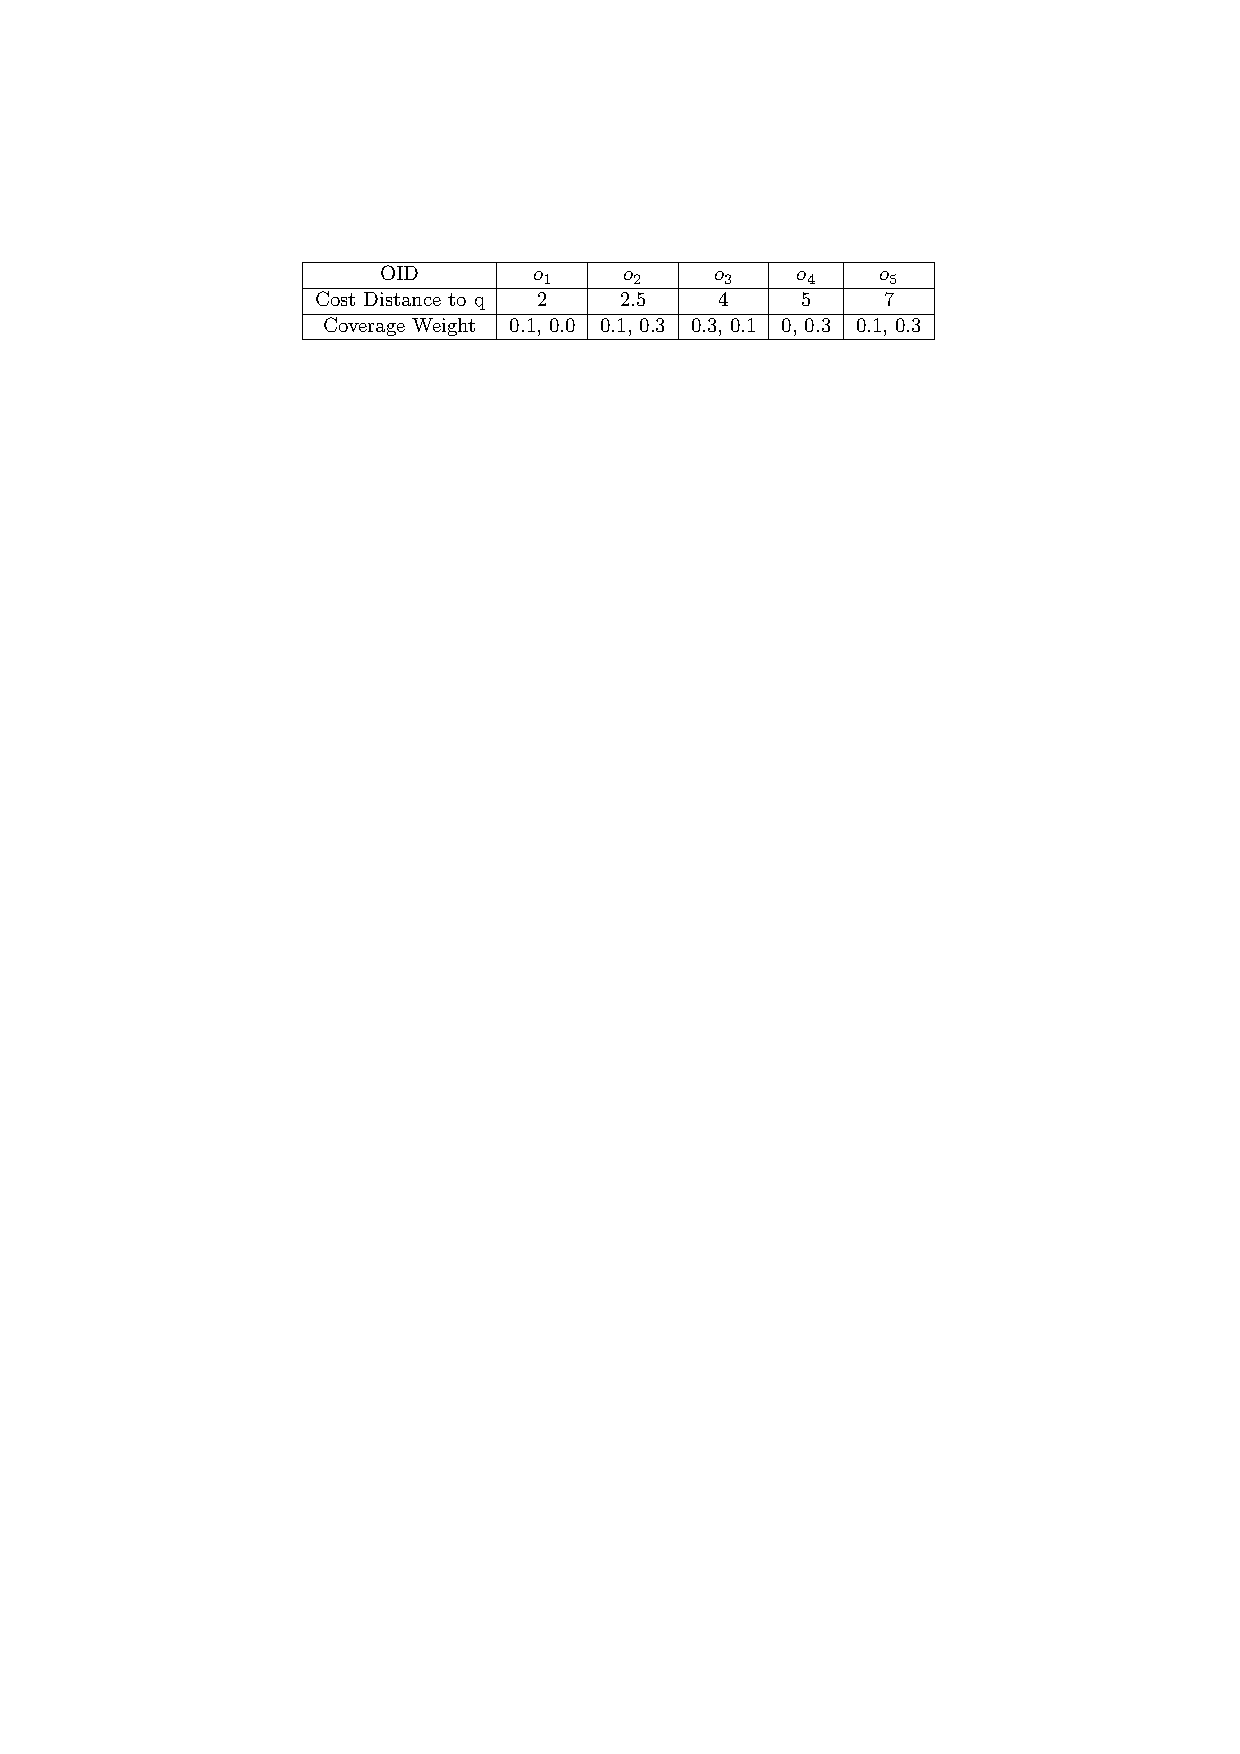
\includegraphics[width=3in,height=0.5in]{MergeList-Q}
    }
    \subfigure[] { \label{MergeList-S}
    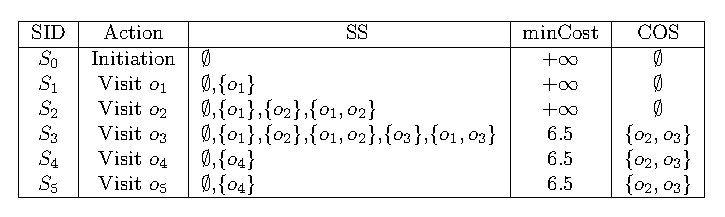
\includegraphics[width=3in,height=1.2in]{MergeList-S}
    }
\caption{An example of MergeList}
\label{F30}
\end{figure}

\textbf{Example 3}: Consider a query q with two keywords $q.\omega=\{\lambda_1, \lambda_2\}$. Fig. \ref{F30}a illustrates the $RO_q$ and the cost distance to q and the corresponding coverage weight. We illustrate the process of MergeList in Fig. \ref{F30}b. There are total six steps to answer this query.
\begin{itemize}
    \item Step 1 (Initiation): We initiate the $SS$, $minCost$ and $COS$ in this step.
    \item Step 2 (Visit $o_1$): Due to $RO_q$ in Fig. \ref{F30}a has been sorted, we visit the object according to the order in Fig. \ref{F30}a We first visit $o_1$, and merge it with ecs in $SS$.
    \item Step 3 (Visit $o_2$): Object $o_2$ is merged with ecs in $SS$.
    \item Step 4 (Visit $o_3$): In this step, we obtain a feasible solution $COS=\{o_2,o_3\}$. And to filter candidate sets with Lemma 4.
    \item Step 5 (Visit $o_4$): In this step, ecs which satisfies Lemma 4 is pruned by COS.
    \item Step 6 (Visit $o_5$): Because the cost of $o_7$ is larger than $minCost$, so Lemma 3 is met and COS is the optimal solution.
\end{itemize}

%\begin{table}[h]
%\centering
%\begin{tabular}{|c|c|p{2cm}|c|c|}
%\hline
% SID & Action & SS & minCost & COS\\
%\hline
%$S_0$ & Initiation & $\emptyset$ & $+\infty$ & $\emptyset$\\
%$S_1$ & Visit $o_1$ & $\emptyset$,\{$o_1$\} & $+\infty$ & $\emptyset$\\
%$S_2$ & Visit $o_2$ & $\emptyset$,\{$o_1$\},\{$o_2$\},\{$o_1,o_2$\} & $+\infty$ & $\emptyset$\\
%$S_3$ & Visit $o_3$ & $\emptyset$,\{$o_1$\},\{$o_2$\},\{$o_1,o_2$\},\{$o_3$\},\{$o_1,o_3$\} & 6.5 & \{$o_2,o_3$\}\\
%$S_4$ & Visit $o_4$ & $\emptyset$,\{$o_4$\} & 6.5 & \{$o_2,o_3$\}\\
%$S_5$ & Visit $o_5$ & $\emptyset$,\{$o_4$\} & 6.5 & \{$o_2,o_3$\}\\
%\hline
%\end{tabular}
%\caption{The process of MergeList} \label{T7}
%\end{table}

\begin{thm}
    (Correctness of MergeList): The MergeList algorithm always produce the correct result set.
    \begin{pot}
        Assuming the number of objects in $RO_q$ is n, hence, there are up to $2^n-1$ candidate sets. Each ecs either used to update the $COS$ or pruned by the $COS$. If the cost of ecs less than $minCost$, we take ecs as our $COS$. Otherwise, we prune ecs and any superset of it. Hence, it is suffice to show that MergeList never prune any feasible solution whose cost less than $minCost$ (false negatives), and never maintain the ecs whose cost larger than $minCost$ (false positives). So the MergeList algorithm always produce the correct result.
    \end{pot}
\end{thm}











